
% 和文概要
\begin{abstract}
実世界と情報世界を接続し,大学の研究室内での情報共有を便利にするシステムを作成した.本システムには3つの機能がある.1つ目の機能は,物体を識別する機能である.研究室内では各人が共有物を使って工作や勉強を行っている.また,私物を持ち込む場合もある.しかしそれらの物品は小型な場合が多く,RFIDやバーコードなどのタグを付けると実際の作業の邪魔になってしまう.そこで本研究では,重さを用いて物体を認識するしくみを作成した.2つ目の機能は,物に対してweb上から複数人で情報を付与する機能である.研究室内にある機材には付箋や書き込み以上の注釈を書きたい場合もあるし,写真や映像で使い方を説明したい事もある.3つ目の機能は,web上での情報更新を実世界に通知する機能である.私たちは常にラップトップコンピュータを開いているわけではなく,移動したり,他の作業をしていたりする.一般的に研究室の全員に情報を共有する方法としてメーリングリストを使う事が多いと思うが,そうではなくweb上の情報を主として,その更新通知のみを行うもっと軽い方法が必要だと考えた.
\end{abstract}

% 英文概要
\begin{eabstract}
english english english
\end{eabstract}

\maketitle

% 本文はここから始まる
\section{はじめに}\label{sec:Introduction}
実世界と情報世界を接続する時に,主に3つの問題がある.物とweb上の知識のリンク方法と,web上でいかに知識を共同編集するかという事,そしてその更新をユーザーにどのようにして通知するかという事である.本論文で説明するシステムでは,大学の研究室という環境において工具や道具などの物体からweb上の知識へと簡単にリンクさせる事ができ,またweb上での知識を共同編集し,その編集過程を研究室のメンバーにリアルタイムに通知する事ができる.

大学の研究室にある特殊な工具についての情報をweb上の情報とリンクさせる際に,まずユーザにとって物の正確な名前がわからないので検索できない事が問題になる.その問題を解決する方法として,
(ここに関連研究.バーコードの例,RFIDの例,画像検索の例,お茶大のWISS)
本研究では,物の持つ物理的な特徴である重さを用いて,物体を認識する事にした.物体認識に重さを使う事には以下の2つの利点がある.1つ目は,使いやすい事である.バーコードの様に正しい向きでスキャンする必要が無く,ただはかりに乗せるだけで良い.また画像検索と異なり正面を向けて置く必要もない.2つ目は,物体が最初から持っている物理的特徴を利用するので,タグ等を貼り付ける必要が無い事である.

web上での知識の共同編集方法の代表的な物としてはwikiが挙げられる.MediaWiki\cite{mediawiki}等のwikiには更新通知機能があるが,その通知方法はメールで定期的にまとめて通知されるものである.しかし,研究室のメンバーはそれぞれがパソコンに向かっていたり,移動していたり,電子工作をしていたりする.つまり既存のwikiとその更新通知システムでは,多様な状態を持つユーザに対してリアルタイムな更新通知ができない.本研究では,webサービスとして実装されたアウトラインエディタと,様々なメディアに適切なフォーマットで更新通知するシステムにより,この問題を解決した.


\section{システムの概要}
本システムには,1.重さにより物体を認識する機能,2.物についてweb上で文書を共同編集する機能,3.web上の文書の更新をユーザに適切に通知する機能 がある.ここでは,実装したシステムの使い方について説明する.

\subsection{はかり}

ユーザは研究室内にある工具や道具をはかりに乗せる.(図:\ref{fig:sensor})はかりは重さを計測し,物体と重さのデータベースを検索する.該当する重さが存在すれば,はかりが接続されたコンピュータにウェブブラウザが表示される.データベース上に該当する物体が無ければ,新しく名前を付ける画面が表示される.

\begin{figure}
  \begin{center}
    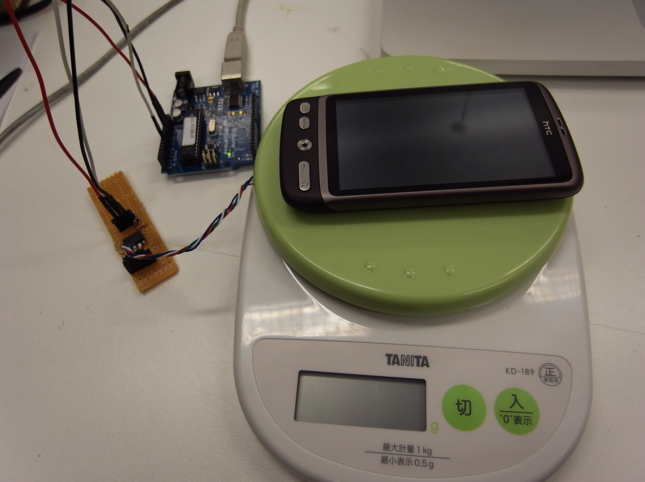
\includegraphics[height=50mm]{img/sensor.png}
  \end{center}
  \caption{重さを計るセンサーの試作版}
  \ecaption{prototype of sensor to detect weight}
  \label{fig:sensor}
\end{figure}

\subsection{gyaazz}

ウェブブラウザ上ではgyaazzというアウトラインエディタが表示される(図:\ref{fig:gyaazz})gyaazzはgyazz\cite{gyazz}を参考にして実装されたウェブアプリケーションである.マウスでクリックした行を画面遷移する事無くその場で編集でき,[と]の記号のみを用いたマークアップで簡潔に画像やリンクなどを挿入できる.emacs風のキーボードショートカット機能を持ち,アウトラインエディタとしてのブロック単位の編集が容易になるようにデザインされている.複数のユーザが同時に1つのページを編集した場合も,編集内容は自動的に同期される.ユーザはこのgyaazz上で物に関する情報を記述する.

\begin{figure}
  \begin{center}
    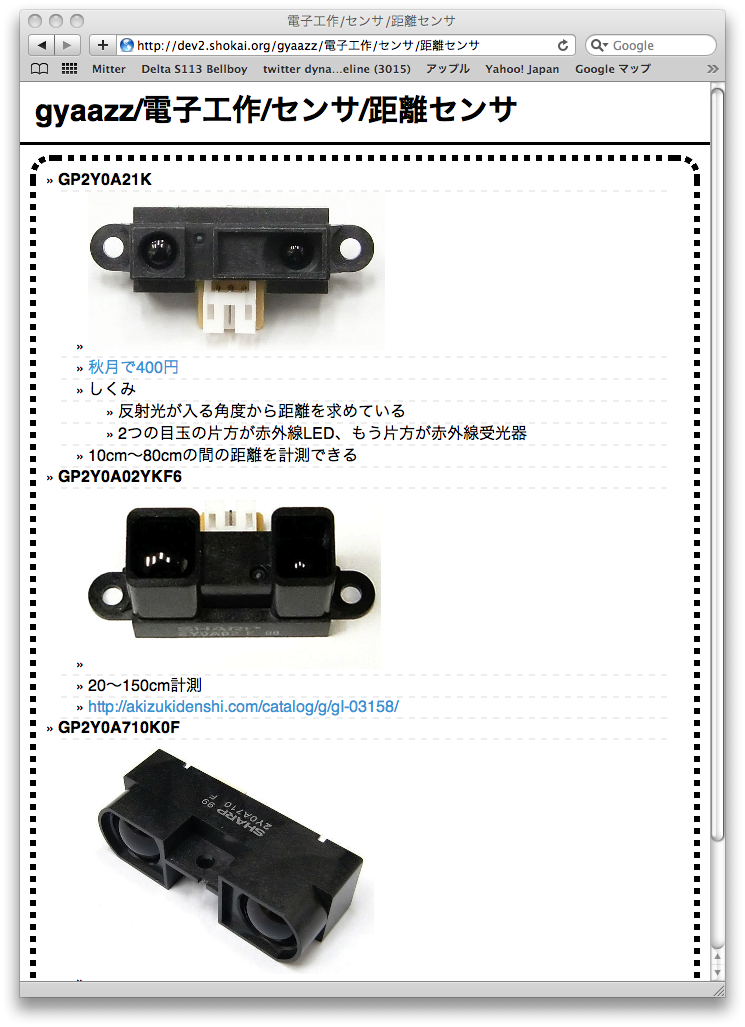
\includegraphics[height=100mm]{img/gyaazz.png}
  \end{center}
  \caption{ウェブアプリケーション gyaazz}
  \ecaption{gyaazz : outline editor web application}
  \label{fig:gyaazz}
\end{figure}

\subsection{gyazz-checker}

gyazz-checkerはgyaazz上での編集をリアルタイムに他のユーザに更新通知できるツールである.gyazzおよびgyaazzの更新を,パソコン上のインスタントメッセンジャー,スマートフォン,twitterに通知できる.gyaazzはアウトラインエディタなので,更新の差分は行毎になる.gyazz-checkerは数分おきにページの上から順に行毎に差分を取り,変更があった行と新規挿入された行をユーザに通知する.この行毎の差分が様々なメディアでの表示に容易に最適化できる事が重要である.

gyazz-checkerはパソコン上で使うインスタントメッセンジャーに対しては,全ての変更を通知する.5秒間隔で1行毎に送信する事で,まるでチャットの様に受信される.(図:\ref{fig:checker})また通知にはim.kayac.com\cite{imkayac}も対応していて,iPhoneやAndroid等のスマートフォンにもpush通知を行うことができる.

gyazz-checkerにtwitterアカウントを設定しておくと,そのアカウントにも更新通知が行われる.(図:\ref{fig:twitter})しかしtwitterに全ての差分の通知を行うとタイムラインがgyazz-checkerで埋まってしまう.研究室メンバーはそれぞれtwitter上で300から2000人をfollowしている.メンバーが煩わしさを感じずにgyaazz上の更新の盛り上がりをtwitter上でも感じられる様に調整した結果,1ページ毎に1行から3行を10分毎にtwitterに通知する事にした.

\begin{figure}
  \begin{center}
    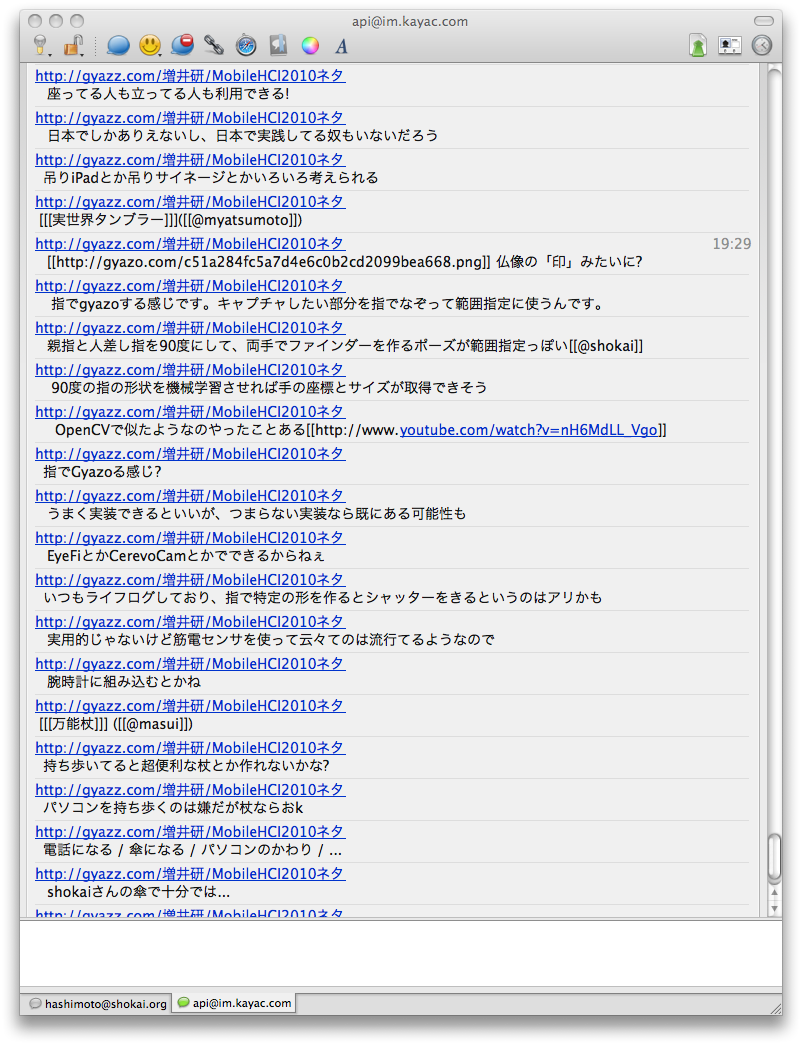
\includegraphics[height=80mm]{img/gyazz-checker.png}
  \end{center}
  \caption{google talk上でのgyazz-checker}
  \ecaption{gyaazz-checker on google talk}
  \label{fig:checker}
\end{figure}

\begin{figure}
  \begin{center}
    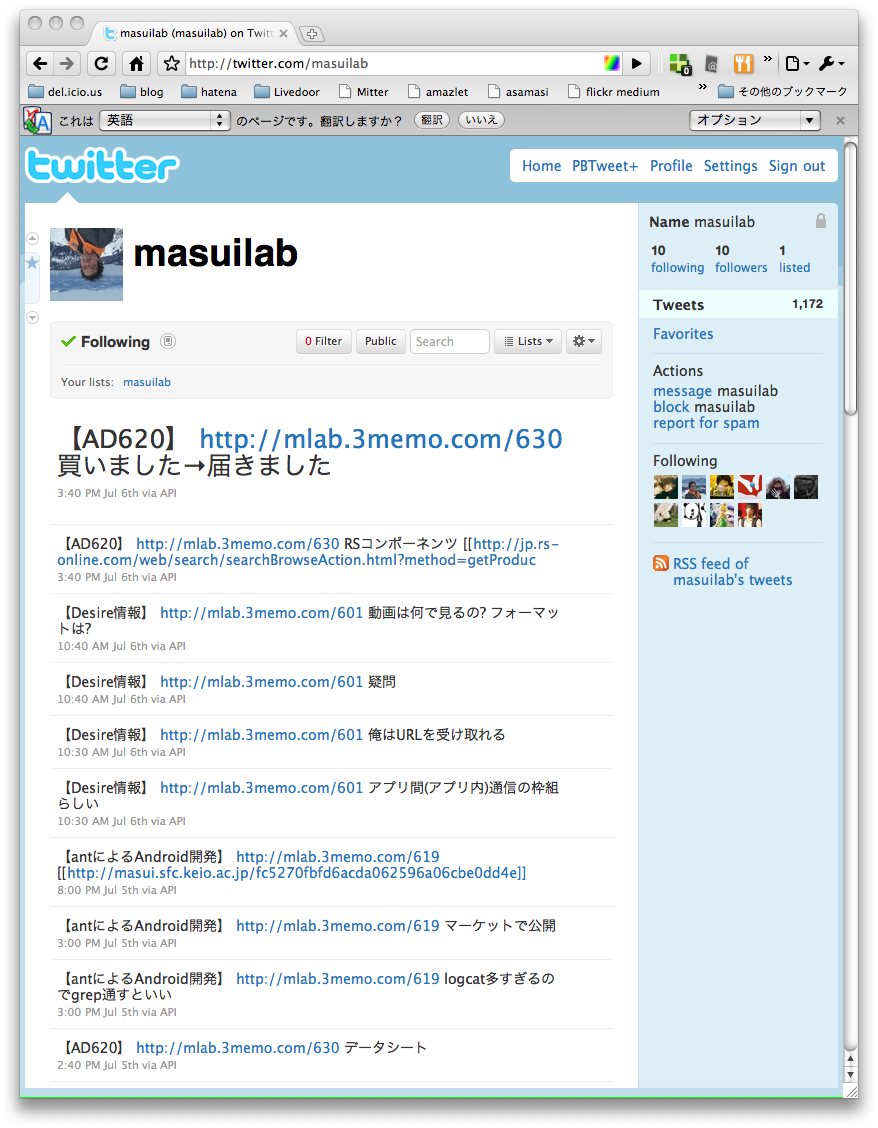
\includegraphics[height=90mm]{img/gyazz-twitter.png}
  \end{center}
  \caption{twitter上でのgyazz-checker}
  \ecaption{gyaazz-checker on twitter}
  \label{fig:twitter}
\end{figure}

\section{システムの実装}
本システムは2章で説明した通り,はかりとアウトラインエディタと更新通知システムの3つに分けられる.この章では3つを順に説明する.

\subsection{はかりの実装}
ストレンゲージは体重計やキッチンスケールに使われる部品である.金属製の角棒の2面に抵抗が貼りつけられていて,棒のわずかなしなりに伴い貼りつけられた抵抗も伸縮する.2つの抵抗値の差分を計測する事で,物の重さをはかる事ができる.

ストレンゲージはタニタ社製キッチンスケール KD-189を分解して取得した.オペアンプAD620BNZで差動増幅回路を組み,その出力をArduino\cite{arduino}の10bitADコンバータで計測する.AD620BNZのゲイン設定用抵抗には温度係数の小さい巻線抵抗を使用する事で,気温の変化による誤差を小さくする事ができた.計測値をUSBケーブルでパソコンに送信し,パソコン上のRubyスクリプトで100回分の平均と値の標準偏差を取得する.パソコン上のプログラムは,初回起動時に10グラム,20グラム,30グラムの重さの分銅を乗せて値を学習させる事でキャリブレーションが行える.ストレンゲージ毎に個体差があるが,約0.5グラム単位で重さを計測する事ができた.100回分の重さの標準偏差が0.5グラム以下の時,物体がはかりの上で静止していると認識し,重さと物体のデータベースに問い合わせる.データベースはkey-valueストアであるMongoDB\cite{mongodb}と,RubyのウェブアプリケーションフレームワークであるSinatra\cite{sinatra}で実装されていて,HTTPとJSONによるRESTfulなAPIで扱うことができる.重さデータベースは重さに対して適切なgyaazzページのURLを返すので,それをパソコン上のウェブブラウザで表示する.

\subsection{gyaazzの実装}
gyaazzはSinatraで実装したウェブアプリケーションで,データベースにはTokyo Cabinet\cite{tc}を利用した.UIはjQuery\cite{jQuery}を利用してJavaScriptで実装した.クリックした行毎にマウスイベントを割り当ててあり,HTMLをformタグに書き換える事で行ごとの画面遷移なしの編集を実現している.キーボードの上下左右キーおよびemacs風のctrlキーとp,n,b,f,a,eキーを同時に押す事により,カーソルが移動する.編集中の行でctrlキーと上下左右キーを同時に押すことで,その行を上下の行と入れ替えたり,インデントする事ができる.shiftキーと同時に押すとアウトラインエディタとしてブロック毎に入れ替えたり,インデントを変更できる.
ユーザが20秒間操作していないか,ウェブブラウザのウィンドウが非アクティブになった時に行の編集状態が解除される.この時サーバーと通信してデータを保存し,ウェブブラウザ上の表示もサーバーから取得した最新の物に更新する.これにより,複数人での同時編集が可能となっている.

\subsection{gyazz-checkerの実装}
gyazz-checkerはRubyスクリプトで実装されたツールで,gyazzおよびgyaazzのページを全件取得し,更新のあったページとその内容をスマートフォンやインスタントメッセンジャー,twitterに通知する.取得したページはTokyo Cabinetに時刻をキーとして蓄積され,一回前の取得データと

wikiの更新は定期的にtwitterとiPhoneとAndroidとIMに流れる.便利!!
githubへのリンクを貼りまくろう.はかりとか更新通知の精度・速度については適当に書く.


\section{まとめ}
重さで物体認識してweb上の情報と関連付け,wikiも作って,通知機能も作った.便利である.


\begin{thebibliography}{10}

\bibitem{mediawiki}
MediaWiki. http://www.mediawiki.org

\bibitem{gyazz}
Gyazz. http://gyazz.com

\bibitem{imkayac}
im.kayac.com. http://im.kayac.com

\bibitem{arduino}
Arduino. http://arduino.cc

\bibitem{mongodb}
MongoDB. http://www.mongodb.org

\bibitem{sinatra}
Sinatra. http://www.sinatrarb.com

\bibitem{jQuery}
jQuery. http://jquery.com

\bibitem{tc}
TokyoCabinet. http://fallabs.com/tokyocabinet/

\end{thebibliography}

